\documentclass{article}
\usepackage{graphicx} % Required for inserting images
\usepackage[top=0.9in, bottom=1in, left=1.5in, right=1.5in]{geometry}
\usepackage[utf8]{inputenc}
\usepackage[icelandic]{babel}
\usepackage[T1]{fontenc}
\usepackage[sc]{mathpazo}
\usepackage[parfill]{parskip}
\renewcommand{\baselinestretch}{1.2}
% Tables and lists
\usepackage{booktabs,tabularx}
\usepackage{multirow}
\usepackage{enumerate}
\usepackage{adjustbox}
\usepackage{multicol}
\usepackage{xcolor}
\usepackage{algpseudocode}
\usepackage{tikz}
\usepackage{nicefrac}
\usepackage{changepage}
\usetikzlibrary{arrows, positioning, calc, graphs}

% Math
\usepackage{amsmath, amsfonts, amssymb, amsthm}
% Graphics

\usepackage{graphicx}
\usepackage{tikz}
% Code environment
\usepackage{minted}
%\usepackage{bm}
%\usepackage{siunitx}
%\usepackage{animate}
%\usepackage{hyperref}
%\usepackage{movie15}
%\usepackage{multicol}
%\usepackage{changepage}
\title{Forritunarmál Einstaklingsverkefni 4}
\author{Ragnar Björn Ingvarsson, rbi3}
\tikzset{->, >=stealth', shorten >=1pt, node distance=2cm,thick, main node/.style={circle,draw,minimum size=3em}}

\begin{document}
\renewcommand\thepage{}
	
	\maketitle

	\newpage
	\setcounter{page}{1}
	\renewcommand\thepage{\arabic{page}}

	\section{}
	\begin{verbatim}
;; Notkun: (sum1 n)
;; Fyrir: n er heiltala, n>=0
;; Gildi: Summan 0+1+...+n
(define (sum1 n)
  (define (sum1help n total)
	(if (= n 0)
		(+ n total)
		(sum1help (- n 1) (+ total n))
		)
	)
  (sum1help n 0)
  )
	\end{verbatim}

	\begin{center}
		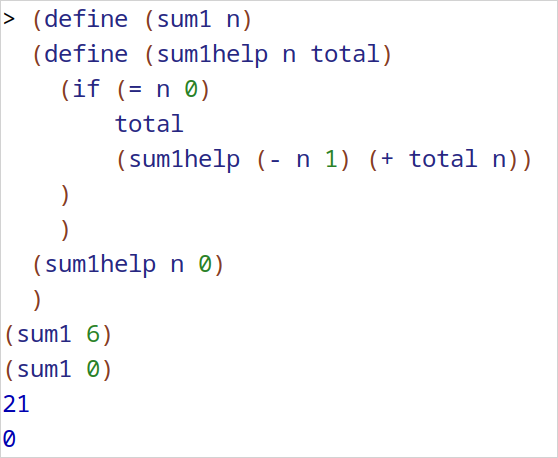
\includegraphics[scale=0.35]{sum1.png}
	\end{center}

	\newpage
	\section{}
	\begin{verbatim}
;; Notkun: (sum2 i n)
;; Fyrir: i og n eru heiltölur, i <= n+1
;; Gildi: Summan i+(i+1)+...+n, summa þeirra
;; heiltalna k þannig að i <= k <= n.
(define (sum2 i n)
  (define (sum2help i n total)
    (if (= i (+ n 1))
        total
        (sum2help (+ i 1) n (+ i total))
        )
    )
   (sum2help i n 0)
  )
	\end{verbatim}
	\begin{center}
		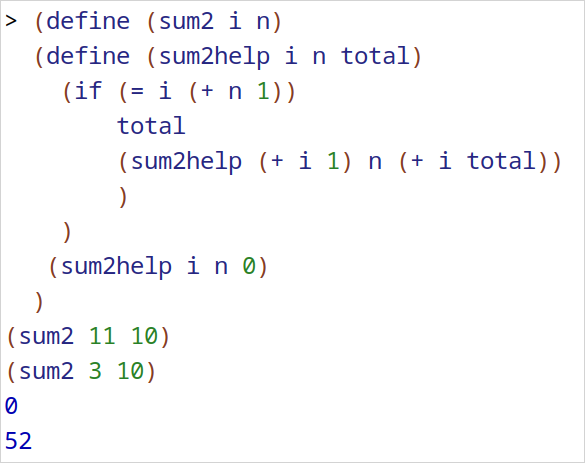
\includegraphics[scale=0.35]{sum2.png}
	\end{center}

	\newpage
	\section{}
	\begin{verbatim}
;; Notkun: ((sum3 i) n)
;; Fyrir: i og n eru heiltölur, i <= n+1
;; Gildi: Summan i+(i+1)+...+n
(define (sum3 i)
  (lambda (x) (if (= i (+ x 1)) 0 (+ i ((sum3 (+ i 1)) x))))
  )
	\end{verbatim}
	\begin{center}
		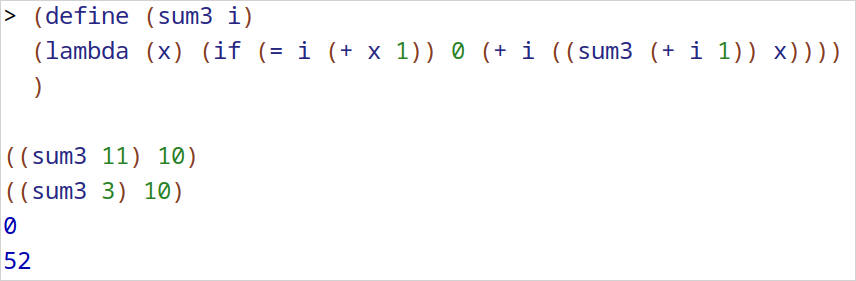
\includegraphics[scale=0.35]{sum3.png}
	\end{center}

	\newpage
	\section{}
	\begin{verbatim}
;; Notkun: (reviota n)
;; Fyrir: n er heiltala n >= 0
;; Gildi: (n n-1 ... 2 1)
(define (reviota n)
  ;; Notkun: (helper m l)
  ;; Fyrir: m er heiltala 0 < m <= n+1, l er listi
  ;; Gildi: (n n-1 ... m+1 m)
  (define (helper m l)
    (if (= m (+ n 1))
        l
        (helper (+ m 1) (cons m l))
        )
    )
  (helper 1 '())
  )
	\end{verbatim}
	\begin{center}
		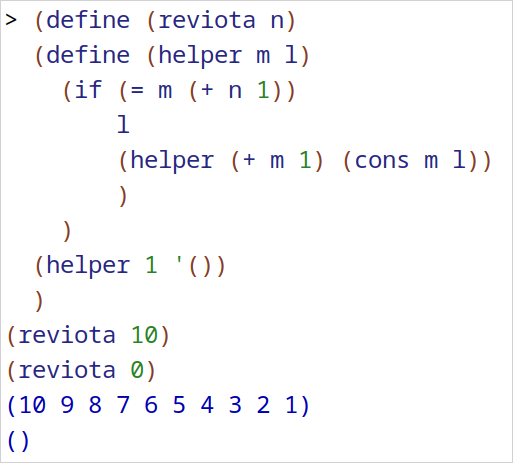
\includegraphics[scale=0.35]{reviota.png}
	\end{center}

\end{document}
